\subsection{Framework} \label{framework}
\begin{figure}[H]
	\centering
	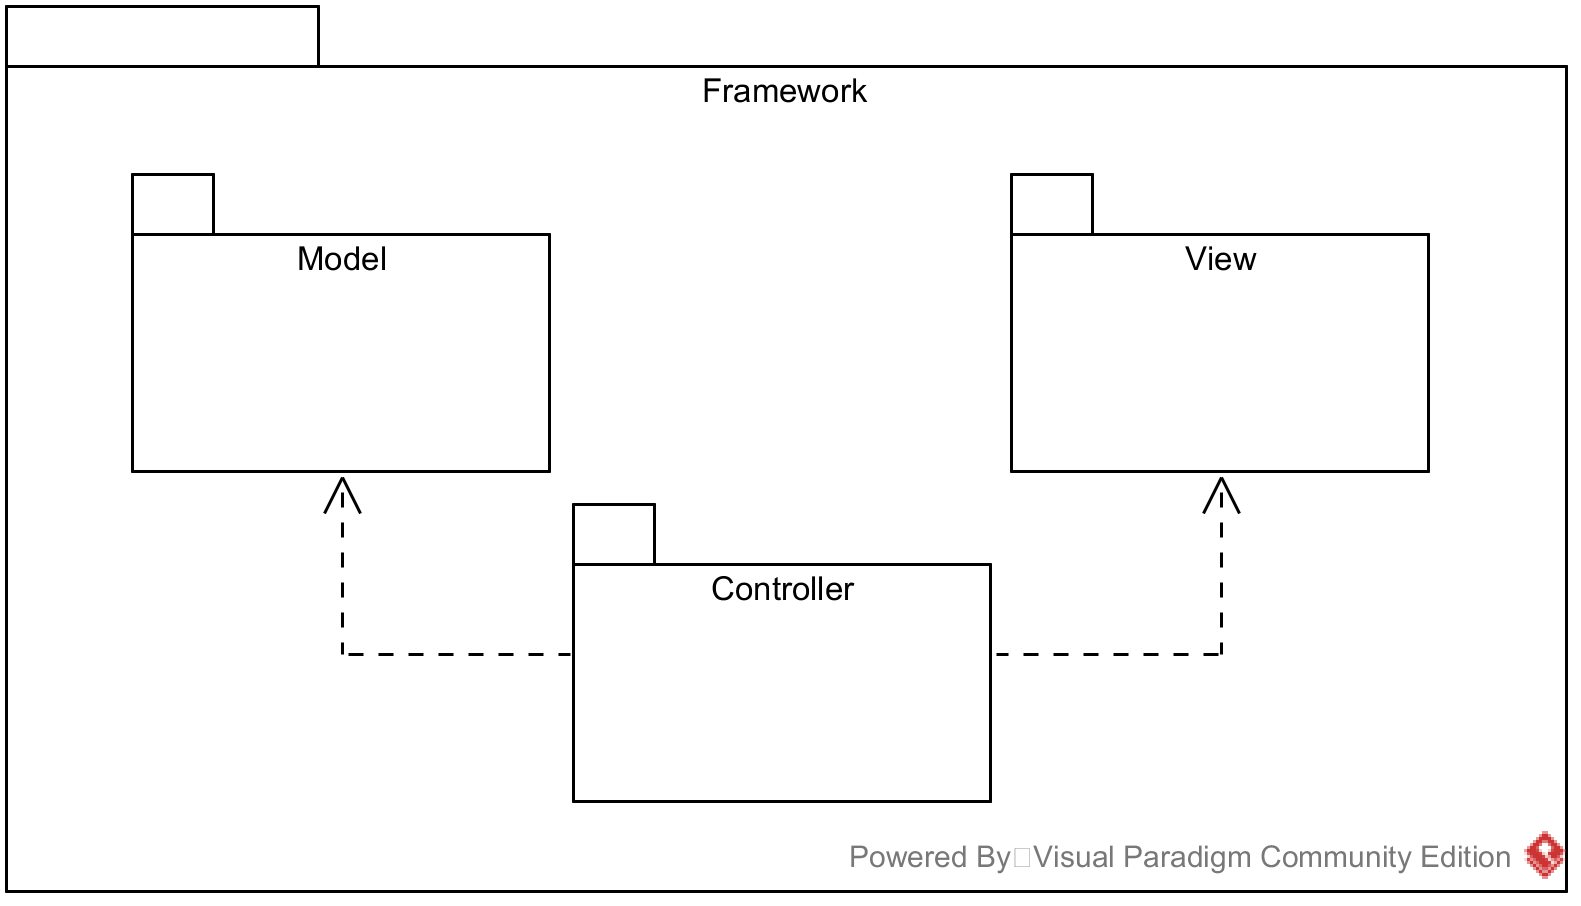
\includegraphics[width=15cm]{./diagrammi/framework.png}
	\caption{Componente Framework}
\end{figure}
\glossario{Framework} è il \glossario{package} base per la corrispondente parte di progetto. È composto dai package Model, View e Controller, in relazione tra loro secondo il \glossario{design pattern} adottato \glossario{MVC}, nella sua versione pull.

\setclass{Framework::Model}
\subsubsection{\class} \label{\class}
\begin{figure}[H]
	\centering
	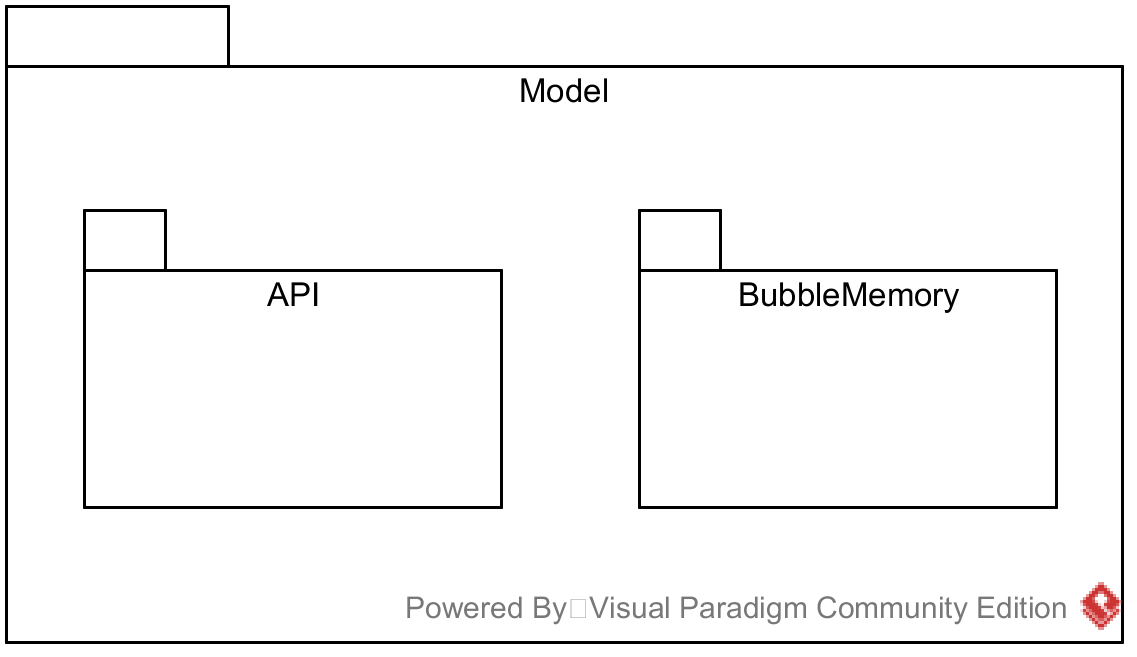
\includegraphics[width=10cm]{./diagrammi/framework/model.png}
	\caption{Componente Framework::Model}
\end{figure}
Contiene la business logic del framework, ed è composto dai package API e BubbleMemory.

\setclass{Framework::Model::API}
\paragraph{\class}\mbox{}\\ \label{\class}
\begin{figure}[H]
	\centering
	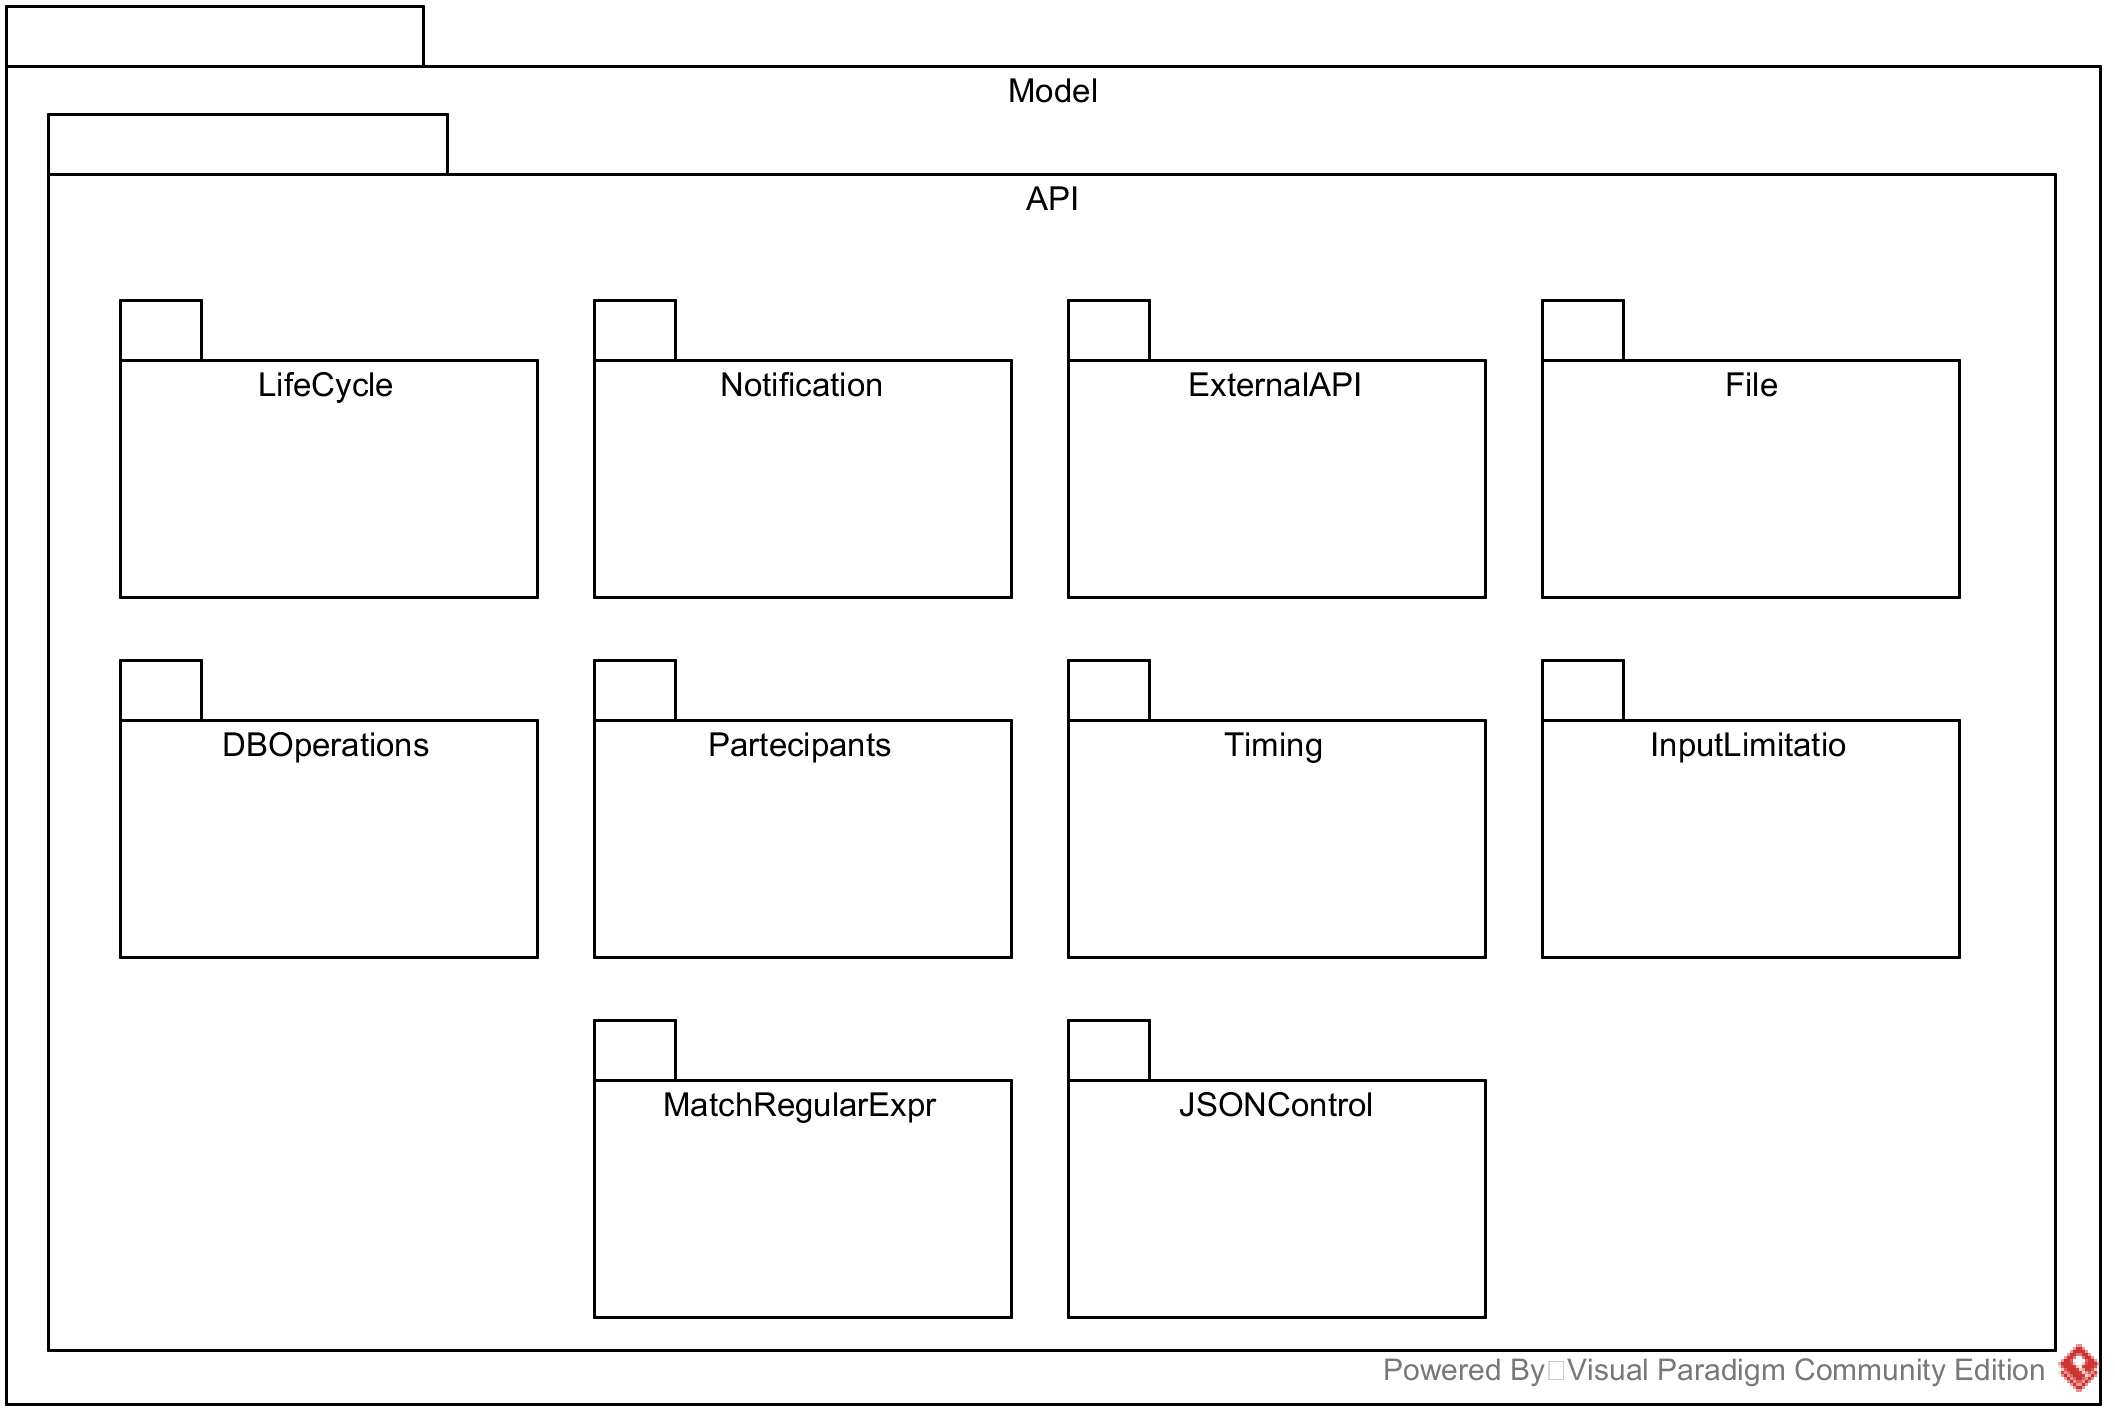
\includegraphics[width=15cm]{./diagrammi/framework/model/api.png}
	\caption{Componente Framework::Model::API}
\end{figure}
Questo componente ha lo scopo di racchiudere in sè tutte le funzionalità logiche offerte dal framework. Non vi sono relazioni tra esse per mantenere una forte indipendenza.

\setclass{Framework::Model::API::LifeCycle::LifeCycle}
\subparagraph{\class}\mbox{}\\ \label{\class}
\begin{figure}[H]
	\centering
	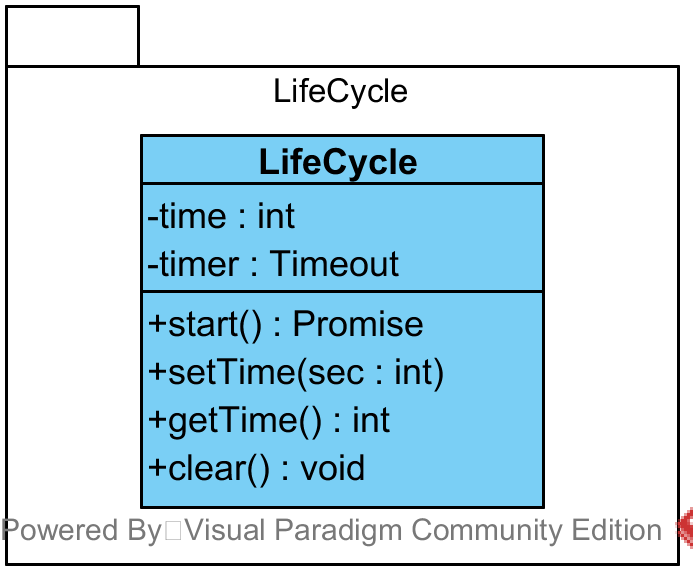
\includegraphics[width=7cm]{./diagrammi/framework/model/api/lifecycle.png}
	\caption{Classe Framework::Model::API::LifeCycle::LifeCycle}
\end{figure}

\textbf{Descrizione:}\\
Classe che permette di inizializzare e avviare un timer.

\textbf{Utilizzo:}\\
Viene utilizzata per definire il tempo di vita di una bubble e avviare il timer che ne determina la fine.

%\textbf{Classi ereditate:}

%\textbf{Sottoclassi:}

\textbf{Attributi:}
\begin{itemize}
	\item \code{- time: int}: durata in secondi del timer;
	\item \code{- timer: Timeout}: riferimento al timer.
\end{itemize}

\textbf{Metodi:}
\begin{itemize}
	\item \code{+ start(): Promise}: restituisce una promise in cui il timer viene avviato;
	\item \code{+ getTime(): int}: restituisce il tempo impostato;
	\item \code{+ setTime(sec: int): void}: permette di settare il tempo:
	
%	Questa riga vuota è importante per il layout
	\indent\textbf{Parametri:}
	\begin{itemize}
		\item \code{sec: int}: durata in secondi del timer.
	\end{itemize}
	\item \code{+ clear(): void}: permette di fermare il timer e resettarlo.
\end{itemize}

\setclass{Framework::Model::API::Notification::WebNotification}
\subparagraph{\class}\mbox{}\\ \label{\class}
\begin{figure}[H]
	\centering
	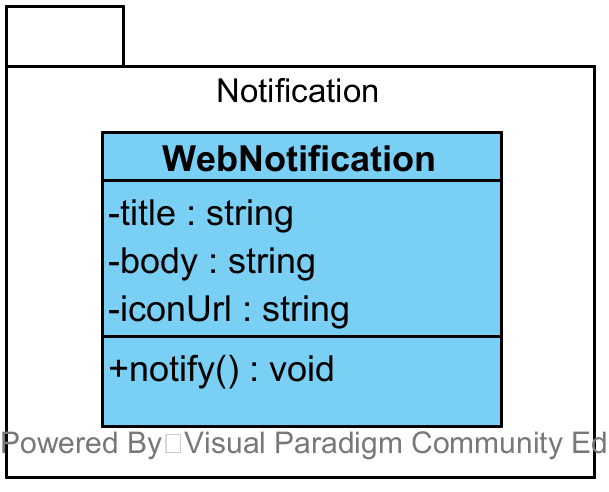
\includegraphics[width=7cm]{./diagrammi/framework/model/api/notification.png}
	\caption{Classe Framework::Model::API::Notification::WebNotification}
\end{figure}

\textbf{Descrizione:}\\
Classe che permette di creare notifiche.

\textbf{Utilizzo:}\\
Viene utilizzata per creare e mostrare delle notifiche all'utente utilizzatore della bubble.

%\textbf{Classi ereditate:}\\

%\textbf{Sottoclassi:}\\

\textbf{Attributi:}
\begin{itemize}
	\item \code{- title: string}: titolo della notifica;
	\item \code{- body: string}: messaggio della notifica;
	\item \code{- iconUrl: string}: URI dell'icona della notifica.
\end{itemize}

\textbf{Metodi:}
\begin{itemize}
	\item \code{+ notify(): void}: se sono state attivate, crea una notifica.
\end{itemize}

\setclass{Framework::Model::API::ExternalAPI::ExternalAPI}
\subparagraph{\class}\mbox{}\\ \label{\class}



